\chapter{ATIVIDADES DESENVOLVIDAS}
\vspace*{-2cm}

O CELTAB tem um projeto solicitado pela Itaipu, de otimização do software que já esta em uso de documentação e organização de coleta e analise amostras de aguá e outros organismos, como microrganismos e algas.

O primeiro passo para o desenvolvimento desta ferramenta, é a confecção do banco de dados onde estes registros irão armazenados e para isso primeiramente é preciso realizar uma analise dos dados que estão armazenados.

\section{Analise dos dados}

Um planilha foi enviada e foi verificado que continha quatro abas, e cada tem uma destas abas um tipo de registro especifico. A primeira aba tem identificação de "Parâmetro de analise", esta aba possui medições química e físicas da aguá e serve como parâmetro de analise para as outras abas:
\begin{itemize}
\singlespacing
\item   Estação: Identificação da coleta/amostra
\item   Ponto de Coleta, Município, Bacia, Corpo Hídrico: Localização da retirada de amostra
\item   Data de Coleta, dia, mês, ano: Quando a amostra foi retirada
\item   Natureza da Amostra, Tipo da Amostra, Campo, Parâmetro: Especificação técnica da amostra (exemplo: Aguá doce sendo uma medição de pH)
\item   Valor: Resultado da analise;
\item   Sigla: sigla de leitura do resultado da medição (exemplo: mg/L, $^{\circ}$C)
\end{itemize}

A terceira e quarta abas é a identificado como "Fito" e "Zoo".

\begin{itemize}
\singlespacing
\item   Estação: Identificação da coleta/amostra
\item   Ponto de Coleta, Município, Bacia, Corpo Hídrico: Localização da retirada da amostra
\item   UTME, UTMN: Coordenadas de localização global (Universal Transversa de Mercator)
\item   Data de Coleta, dia, mês, ano: Quando a amostra foi retirada
\item   Natureza da Amostra, Tipo da Amostra, Campo, Parâmetro: Especificação técnica da amostra (exemplo: Aguá doce sendo uma medição de pH)
\item   Filo, Classe, Ordem, Família, Gênero, Espécie, Valor: Classificação cientifica do organismo que esta sendo medido
\item   Valor: Resultado da analise;
\item   Sigla: sigla de leitura da medição (exemplo: organismos/ml ou células/ml), mas como se trata de uma contagem, todos os registros estão vazios
\end{itemize}

\section{Formas Normais}

De acordo com \cite{wkent}, Formas normais, ou normalização de dados é um conjunto de regras que visa, principalmente, a organização de um projeto de banco de dados para reduzir a redundância de dados, aumentar a integridade de dados e o desempenho.

Para normalizar o banco de dados, deve-se examinar as colunas (atributos) de uma entidade e as relações entre entidades (tabelas), com o objetivo de se evitar anomalias observadas na inclusão, exclusão e alteração de registros.

\subsection{Primeira Forma Normal}

Nesta forma os atributos precisam ser atômicos, o que significa que as tabelas não podem ter valores repetidos e nem atributos possuindo mais de um valor.

\subsection{Segunda Forma Normal}

Primeiramente, para estar na 2FN é preciso estar também na 1FN. 2FN define que os atributos normais, ou seja, os não chave, devem depender unicamente da chave primária da tabela. Assim como as colunas da tabela que não são dependentes dessa chave devem ser removidas da tabela principal e cria-se uma nova tabela utilizando esses dados.

\subsection{Terceira Forma Normal}

Assim como para estar na 2FN é preciso estar na 1FN. 3FN define que todos os atributos dessa tabela devem ser funcionalmente independentes uns dos outros, ao mesmo tempo que devem ser dependentes exclusivamente da chave primária da tabela. 3NF foi projetada para melhorar o desempenho de processamento dos banco de dados e minimizar os custos de armazenamento.

\subsection{Quarta e quinta formas normais}

São formas normais são menos utilizadas, pois não são aplicáveis de forma que melhore o desempenho em todos os domínios, pois nestas formas é para fazer a uma mesma consulta que envolve mais de uma tabela, mais processador.

\subsection{Proposta de modelagem dos dados}

Após a analise dos dados da tabela, foi proposto um modelo que segue os padrões da terceira forma normal, onde, de forma simplificada, foi separado as informações em Data/Hora, Localidade, Identificação e Informações técnicas da amostra, conforme mostrado na imagem \ref{diagramaClasse}

\begin{figure}[!h]
    \centering
    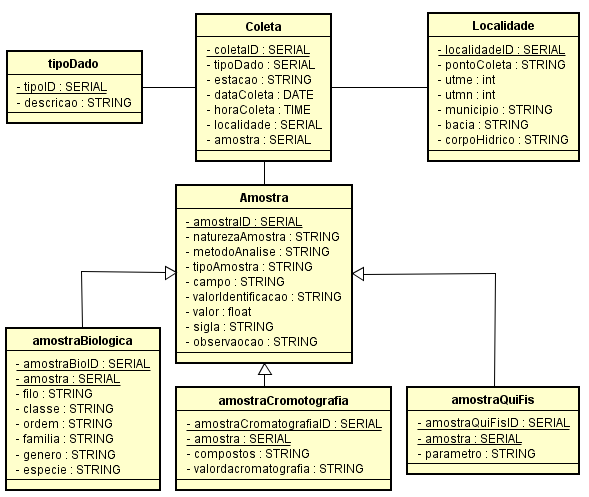
\includegraphics[scale=0.7]{Imagens/Imagens/MER.png}
    \caption{Diagramação do modelo proposto}\label{diagramaClasse}
    \fonte{Autor}
\end{figure}

A herança em banco de dados relacional é feita, utilizando a chave estrangeira como chave primaria, ou seja, o registro amostra identifica o registro especializado.

\section{Importação e conversão}

\subsection{Modelagem e craição do banco de dados}

Segue abaixo o código feito criar o modelo de dados conforme proposto na figura \ref{diagramaClasse}

\lstset{language=SQL}
\begin{lstlisting}[frame=single]
CREATE TABLE localidade (
    localidadeID SERIAL,
    pontoColeta VARCHAR(50),
	utme INT,
	utmn INT,
	municipio VARCHAR(50),
	bacia VARCHAR(50),
	corpoHidrico VARCHAR(50),
	PRIMARY KEY(localidadeID)
);
\end{lstlisting}

\begin{lstlisting}[frame=single]
CREATE TABLE amostra (
	amostraID SERIAL,
	naturezaAmostra VARCHAR(50),
	metodoAnalise VARCHAR(50),
	tipoAmostra VARCHAR(50),
    campo VARCHAR(50),
    valorIdentificacao VARCHAR(50),
	valor FLOAT,
	sigla VARCHAR(50),
	observaocao VARCHAR(50),
	PRIMARY KEY(amostraID)
);
\end{lstlisting}

\begin{lstlisting}[frame=single]
CREATE TABLE coleta (
	coletaID SERIAL,
	tipoDado SERIAL,
	estacao VARCHAR(50),
	dataColeta DATE,
	horaColeta TIME without time zone,
	localidade SERIAL,
	amostra SERIAL,
	FOREIGN KEY(tipoDado) REFERENCES tipoDado(tipoID),
    FOREIGN KEY(localidade) REFERENCES localidade(localidadeID),
	FOREIGN KEY(amostra) REFERENCES amostra(amostraID),
	PRIMARY KEY(coletaID)
);
\end{lstlisting}

\begin{lstlisting}[frame=single]
CREATE TABLE amostraBiologica (
	amostraBioID SERIAL,
	amostra SERIAL,
	filo VARCHAR(50),
	classe VARCHAR(50),
	ordem VARCHAR(50),
	familia VARCHAR(50),
	genero VARCHAR(50),
	especie VARCHAR(50),
	FOREIGN KEY(amostra) REFERENCES amostra(amostraID),
	PRIMARY KEY(amostraBioID, amostra)
);
\end{lstlisting}

\begin{lstlisting}[frame=single]
CREATE TABLE amostraQuiFis (
	amostraQuiFisID SERIAL,
	amostra SERIAL,
	parametro VARCHAR(50),
	FOREIGN KEY(amostra) REFERENCES amostra(amostraID),
	PRIMARY KEY(amostraQuiFisID, amostra)
);
\end{lstlisting}

\begin{lstlisting}[frame=single]
CREATE TABLE amostraCromotografia (
	amostraCromatografiaID SERIAL,
	amostra SERIAL,
	compostos VARCHAR(50),
	valordacromatografia VARCHAR(50),
	FOREIGN KEY(amostra) REFERENCES amostra(amostraID),
	PRIMARY KEY(amostraCromatografiaID, amostra)
);
\end{lstlisting}

\begin{lstlisting}[frame=single]
CREATE TABLE tipoDado (
	tipoID SERIAL,
	descricao VARCHAR(50),
	PRIMARY KEY(tipoID)
);
\end{lstlisting}

\subsection{Algorítimo de importação}

Como as informações vieram de planilhas, foi necessário fazer um algorítimo de reconhecimento e automação da conversão dos dados. Para isso foi necessário criar um construtor que recebesse as informações em um vetor, isso porque quando a torna mais fácil e rápida a reordenação de forma que fique de acordo como o construtor esta esperando.


\begin{table}[h!]
\centering
\caption{Exemplificação do vetor construtor}\label{tabelaExemploConstrutor}
\begin{tabular}{ l | c | c | c | c | r }
Identificador(0) & Data(1) & Hora(2) & Localização(3) & Valor(4) & Sigla(5)
\end{tabular}
\end{table}

Conforma exemplificado na tabela \ref{tabelaExemploConstrutor}, temos varias informações que precisam estar em seus devidos lugares no vetor, pois irá considerar qualquer coisa que estiver em sua posição como informação a ser armazenada, por exemplo, se trocar informações de "sigla" e "identificador" as duas informações ficaram trocadas nos registros finais.

As informações que estão na planilha, nem sempre estão na mesma ordem, comprometendo a utilização direta desta técnica. Para resolver isso foi criado mais um vetor de índices.

\begin{table}[h!]
\centering
\caption{Exemplificação do vetor de índices}\label{tabelaExemploIndices}
\begin{tabular}{ l | c | c | c | c | r }
0(Identificador) & 1(Data) & 2(Hora) & 4(Valor) & 5(Sigla) & 3(Localização)
\end{tabular}
\end{table}

Exemplificando, Na terceira posição do vetor representado na tabela \ref{tabelaExemploIndices} esta armazenado o numero 4, o que significa que o dado que vem da planilha da terceira coluna é dados sobre "Valor", portanto, dentro do vetor construtor precisa ser colocado na quarta posição.